\sloppy
\section{Beschreibung}
\input{einleitung.tex}
\todo{klassen werden kursiv geschrieben }
\label{sec:Allgemeine Beschreibung}
\section{Architektur}
\label{sec:Architektur}
\section{PDF}
\label{sec:PDF}
Das System soll dem Nutzer die Möglichkeit bieten Informationen über einen Raum als PDF zu teilen. Dabei gibt es zwei unterschiedliche PDF‘s, diese beinhalten die generellen Rauminformationen, sowie den dazugehörigen QR-Code oder eine Liste aller Teilnehmer.
Das Android-Framework  verfügt über eine \textit{PdfDocument} Klasse, die zum Erstellen von PDF‘s genutzt wird. Für eine A4 Seite nach DIN Norm ergeben sich die Werte 846x594 Pixel. Näheres zur Berechnung der Pixelwerte ist unter \href{https://developer.android.com/reference/android/graphics/pdf/PdfDocument.PageInfo}{developer.android} zu finden. Die erstellte Seite wird mittels eines Canvas editiert. Die Formatierung  der Texte und Grafikelemente lassen sich über die \textit{Paint} Klasse einstellen.
Das erstellte PdfDokument wird im externen Dateiverzeichnis der App abgespeichert. Der Nutzer besitzt bei einem fehlgeschlagenen Teilen somit trotzdem die Möglichkeit auf das erstellte PDF zuzugreifen.
Um das PDF zu teilen, wird ein FileProvider verwendet, welcher im Manifest deklariert ist.  Der FileProvider bietet dem Nutzer eine Auswahl der installierten Anwendungen, über welche er das PDF teilen kann.

Für die nächste Version der App muss das PDF mit der Übersicht aller Teilnehmer überarbeitet werden. In der aktuellen Version wird die E-Mail Adresse ab einer bestimmten Länge zum Teil mit in die nächste Spalte geschrieben. Ziel ist es, dass ab einer bestimmten Länge ein automatischer Zeilenumbruch in der entsprechenden Spalte stattfindet.

\section{RoomLifecycleService}
\label{sec:RoomLifecycleService}
Der RoomLifecycleService steuert, wie der Name bereits andeutet, in welchem Zustand sich Räume befinden. Er wird ausschließlich im Host-Modus betrieben \todo{passt nicht ganz wird au im participant modus genutzt}.
Die Entscheidung fiel auf einen Service, weil wir auch im nicht-geöffneten Zustand der App auf Nachrichten von außen reagieren wollte. 
Beispiel: Der Host eröffnet einen Raum und wechselt die App oder sperrt das Smartphone. Wenn die Kontaktverfolgungsapp nun nicht mehr im Vordergrund ist während das Timeout ausläuft oder der Raum in die Öffnungszeit reinrutscht, dann würde er nicht geschlossen respektive geöffnet werden. Um also zu vermeiden dass der Host über die gesamt Zeit sein Smartphone nicht verwenden kann und das Display mit hohem Stromverbrauch den Akku entleert haben wir uns für einen Service entschieden. 

Wird der Service gestartet wird die Raumüberprüfungsroutine nebenläufig in einem neuen Thread gestartet. Dadurch verhindern wir dass das der Hauptthread machen muss. Der Raumstatus wird jede Sekunde mit einem Busy-Wait-Algorithmus überprüft. Das sollte man nicht in den Hauptthread auslagern, da er diesen unnötig blockiert. Der Datenbankzugriff ist nicht die Ursache für die Designentscheidung, denn dadurch dass wir schon über das Repository nebenläufig auf die Datenbank zugreifen sind wir bezüglich Datenbank-Latenz bereits auf der sicheren Seite.
Im Thread überprüfen wir initial ob aktuell geschlossene Räume geöffnet und aktuell geöffnete Räume geschlossen werden sollten.
 Nebenher wird im Mainthread versucht den MQTT-Service zu einzubinden. Denn der Host soll natürlich auf alle Räume die sich öffnen hören bzw. aufhören auf alle Räume zu hören die sich geschlossen haben. 
Außerdem muss der Host den Teilnehmern die Raumeigenschaften und den Öffnungsstatus beim Öffnen mitteilen. Wir brauchen den MQTT-Service hier also um Raumstatusänderungen den Teilnehmern mitzuteilen.
Zurück zum LifeCycleService.
Ein Raum hat drei mögliche Zustände:
\begin{enumerate}
\item Wird sich öffnen
\item Geöffnet
\item Geschlossen
\end{enumerate}
 Jede Sekunde wird also überprüft ob Räume die geschlossen sind geöffnet werden sollen, ob Räume die sich öffnen werden geöffnet werden können und ob Räume die geöffnet sind geschlossen werden sollten. 
Falls noch Teilnehmer in zu schließenden Räumen sind werden Sie rausgeworfen. In der Datenbank wird dann für alle Teilnehmer als Austrittszeitpunkt die Timeout-Zeit des Raums eingetragen. 
Auf der Teilnehmerseite reagiert der Observer auf die Änderung des Raumstatuses und beendet den Raum auch real für den Teilnehmer.

\section{RoomTag - QR und NFC}
\label{sec:RoomTag - QR und NFC}
Damit Räume distinktiv sind besitzen Sie einen Identifier. Dieser nennt sich Room-Tag und ist zusammengesetzt aus dem Raumnamen, der Email-Adresse des Hosts und der Id des Raums in der Datenbank der Hostdatei. Beispiel für einen Room-Tags: Vorlesung 1/dozent@hs-mannheim.de/0.
Teilnehmer benötigen diesen Tag um dem Raum beizutreten. Dies können Sie über NFC oder über einen QR-Code durchführen. Eine manuelle Eingabe ist nicht implementiert.

Um den Tag weiterzugeben kann der Veranstalter nach dem erstellen des Raumes ein PDF generieren und per E-Mail versenden. 
Das passiert in der Methode shareRoom() in der Klasse Activity\_22\_RoomHostDetail. 
In einem solchen PDF ist neben Raum-Metadaten wie Titel, Start und End-Zeitpunkt auch ein QR-Code über den die Teilnehmer beitreten können. 
Wir benutzen für die Erstellung die externe Bibliothek zxing von journeyapps unter der Apache 2.0 Lizenz. Wir benutzen dafür die Klasse BarcodeEncoder in der Klasse QRCodeManager.

Ein Schreiben des NFC Codes auf einen NFC Sticker ist nicht implemenentiert.
 Apps wie NFC Tools des Unternehmens wakdev aus dem PlayStore schaffen hier aber Abhilfe. Dort kann der Tag in Plaintext-Format auf den NFC Tag geschrieben werden.
Eine URI sollte nicht vergeben werden, da der Scanner nicht drauf reagieren würde.

Im Laufe der Entwicklung definierten wir fest, dass ein Veranstalter seinen eigenen Raum nicht betreten dürfte. Außerdem sollte ein Teilnehmer, nachdem er eine Sitzung verlassen hatte, nicht wieder erneut teilnehmen dürfen. Damit wurden irreführende Einträge in der Auswertung vermieden. Dieses Verhalten wird mit der Methode checkEnterPeriomission in der Activity\_11\_EnterViaQrNfc abgefangen.
\subsubsection*{Betreten über QR}
\label{subsec: Betreten über QR}
Wünscht der Teilnehmer über QR einzutreten, dann wird in der Activity\_11\_EnterViaQrNfc die Funktion callScanner() aus der QrCodeManager-Klasse gerufen. Dort wird die Scanner-Activitiy aus zxing gestartet, die einen Rückgabewert liefert. Es ist auch möglich den Scanner zu vorkonfigurieren, so, dass z.B. immer der Kamerablitz angeschaltet ist um auch bei schlechten Licht-Bedingungen den QR-Code gut zu erkennen. 
Außerdem kann ein Timeout eingestellt werden, falls der Nutzer den QR Code in einer gewissen Zeit nicht einscanned.
In unserem Projekt wurde sich aber wegen der Benutzerfreundlichkeit gegen diese Konfiguration entschieden.
Der Scanner wird über einen Intent gestartet und liefert wenn er fertig ist ein Ergebnis zurück.
Dieses wird in der Methode onActivityResult verarbeitet. Wenn der Scan geklappt hat wird die Methode enterRoom() aufgerufen. Dort werden die Daten des Room-Tags in die Datenbank eingetragen und die Activity\_14\_RoomParticipantDetail gestartet. Der Teilnehmer hört dort dann auf das korrekte MQTT Topic. Er hat den Raum betreten.
\subsubsection*{Betreten über NFC}
\label{subsec: Betreten über NFC}
Wünscht der Teilnehmer über QR einzutreten, dann wird in der Activity\_11\_EnterViaQrNfc die Funktion armNFCAdapter() aufgerufen. Es wird überprüft ob das Smartphone überhaupt einen NFC Sensor hat.
Falls das erfüllt ist wird dieser auf events des Types ACTION\_NDEF\_DISCOVERED scharfgeschaltet. 
Man sagt auch er ist im Foreground-Dispatch-Modus.
Das bedeutet dass, wenn ein neues NFC Tag detektiert wurde, ein gewisser Intent gestartet wird. 
Falls das der Fall ist, wird die gleiche Activity\_11\_EnterViaQrNfc noch einmal gestartet allerdings mit der Action NFC\_INTENT\_ACTION. 
In der onResume() wird überprüft ob diese Action gesetzt ist, denn nur dann kehrt die Anwendung ja aus dem NFC-Intent zurück. 
In den Extras des NFC-Intents befindet sich dann er abgelesene Room-Tag. Der Ablauf danach ist wie beim Betreten über QR. enterRoom() wird gerufen und Activity\_14\_RoomParticipantDetail wird gestartet.
\section{MQTT-Service}
Der MQTT-Service stellt die MQTT-Funktionalität bereit, über welche die App mit anderen Smartphones kommuniziert.
Das Starten und Stoppen des MQTT-Service findet in der \textit{Activity\_00\_StartActivity} statt. Alle anderen Activities binden lediglich den MQTT-Service. Das Binden des MQTT-Service findet in  \textit{Activity\_11\_EnterViaNfcQr}, \textit{Activity\_14\_RoomParticipantsDetails} und \textit{Activity\_22\_RoomHostDetails} statt. Des Weiteren wird der Service in dem RoomLivecycle-Service gebunden. Näheres hierzu unter \cref{sec:RoomLifecycleService}.  Beim Verwenden des MQTT-Service wird in jeder Activity geprüft, ob dieser schon gebunden ist (not null). Ist dies nicht der Fall, wird das zu sendende Objekt zwischengespeichert und bei erfolgreichem Binden verarbeitet. 
Die im MQTT-Service implementierten Methoden sind ausführlich mittels \href{https://scm.inftech.hs-mannheim.de/gogs/moa/20moagm/src/dev/Doku/javadoc}{JavaDoc} erklärt. 

Die Kommunikation zwischen dem Host und den Teilnehmern verläuft beim MQTT-Protokoll über sogenannte Topics. Für einen Raum werden, wie \cref{img:mqtt} zeigt, immer zwei Topics benötigt. Der Teilnehmer kann einem Raum über die Topic \textit{moagm/Room-Tag} beitreten. Der Host sendet die nötigen Informationen für die Teilnehmer über die Topic \textit{moagm/Room-Tag/public} an alle Teilnehmer. Durch die Trennung der Kanäle wird verhindert, dass Teilnehmer die Nachrichten, welche von anderen Teilnehmern an den Host gesendet werden, empfangen können.

Insgesamt gibt es vier verschiedene Nachrichtentypen, welche zwischen den Teilnehmern und dem Host ausgetauscht werden. Alle Nachrichten werden im JSON-Format versendet. Dabei lassen sich die Nachrichten in zwei Gruppen unterteilen. Die Nachrichten \textit{anmeldung.json} und \textit{abmeldung.json} werden vom Teilnehmer an den Host gesendet. \textit{teilnehmer.json} und \textit{rauminfo.json} sendet der Host an alle Teilnehmer. Mittels eines Converters werden die entsprechenden JSON-Objekte erzeugt und wieder in verwendbare Datentypen zurück gewandelt. Zum Identifizieren eines Nachrichtentyps wird (warum auch immer..) nicht das Typfeld benutzt. 
Das Identifizieren wird mit den folgenden Schlüsselworten durchgeführt.
\begin{description}
\item[•] ENTERTIME (\textit{anmeldung.json})
\item[•] EXITTIME (\textit{abmeldung.json})
\item[•] RAUM (\textit{rauminfo.json})
\item[•] TEILNEHMERLIST (\textit{teilnehmer.json})
\end{description}
Abhängig von dem empfangen Datentyp werden unterschiedliche Aktionen durchgeführt.
\\
Mit der in \cref{lst:anmeldung} dargestellten \textit{anmeldung.json} meldet sich ein Teilnehmer beim Host an und stellt eine Verbindung zu der entsprechenden Topic her. In der Nachricht sind alle relevanten Informationen des Teilnehmers enthalten sowie die Uhrzeit wann er den Raum betreten hat. Der MQTT-Service konvertiert die erhaltene JSON-Nachricht mittels der \textit{AdapterJsonMqtt} Klasse in den passenden Datentyp. Das erhalte \textit{ParticipantItem} Objekt wird in der Datenbanktabelle \textit{dbParticipant} mit der  entsprechenden RaumId abgespeichert. Die entsprechende RaumId kann der Topic entnommen werden, über welche die JSON-Nachricht empfangen wurde. Im Anschluss wird an alle Teilnehmer ein \textit{teilnehmer.json} sowie \textit{rauminfo.json} gesendet.
\begin{figure}
	\centering
	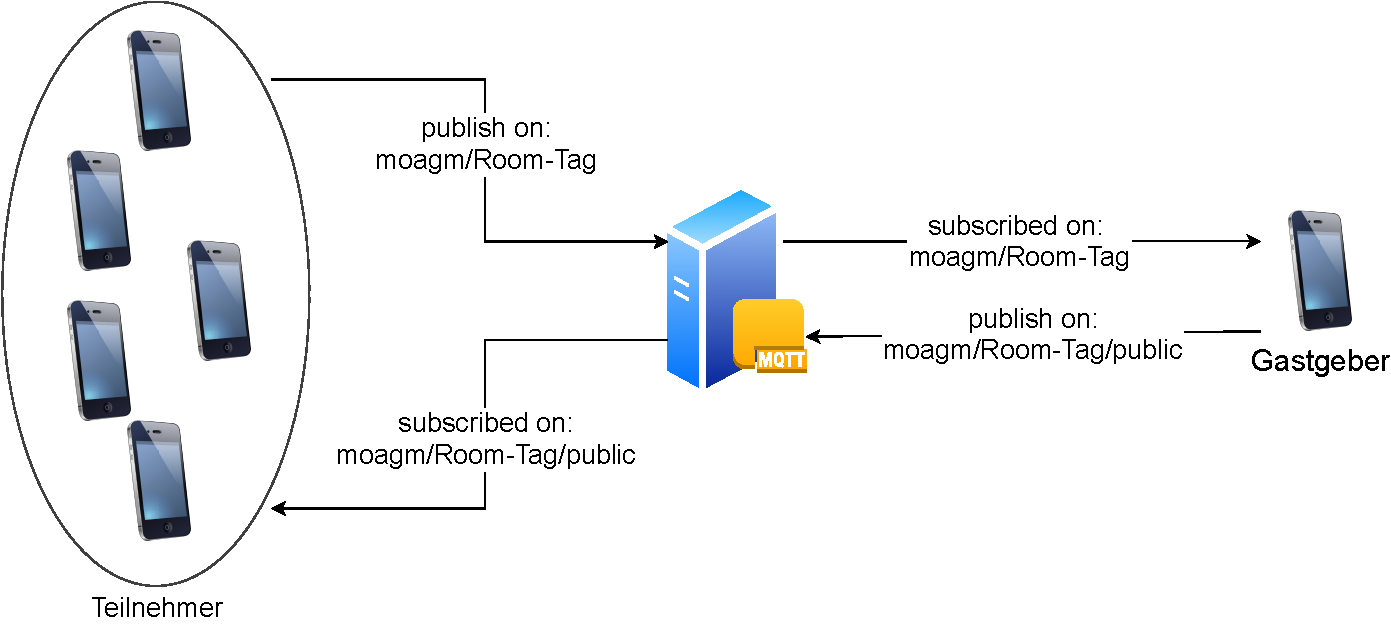
\includegraphics[width =0.8\textwidth]{images/mqttservice.pdf}
	\caption{Darstellung des grundlegenden Kommunikationsablaufes mit MQTT-Topics.}
	\label{img:mqtt}
\end{figure}
Die Nachricht \textit{abmeldung.json}, dargestellt in \cref{lst:abmeldung},   sendet der Teilnehmer an den Host, sobald er den Raum verlässt. Dabei meldet sich der Teilnehmer ebenfalls von der entsprechen Topic der MQTT-Verbindung ab. Analog zum \textit{anmelden.json} enthält diese Nachricht alle wichtigen Informationen über den Teilnehmer sowie die Uhrzeit zu welcher er den Raum verlässt. Im MQTT-Service wird mithilfe des erzeugten \textit{ParticipantItem} Objekt und der RaumId die Exittime des dazugehörenden Teilnehmers aktualisiert.  

\cref{lst:rauminfo} stellt die Nachricht vom Typ \textit{rauminfo.json} da. Diese Nachricht enthält sämtliche Informationen über einen Raum. Jede vom Teilnehmer empfange \textit{rauminfo.json} wird in ein \textit{RoomItem} Objekt konvertiert und in die Datenbanktabelle \textit{dbRoom} eingefügt bzw. aktualisiert den bereits vorhanden Eintrag. Wenn der Host eine \textit{rauminfo.json} versendet, welche den Teilnehmern mitteilt, dass der Raum nun geschlossen ist, meldet der MQTT-Service den Host automatisch von der entsprechenden MQTT-Topic ab.

Der in \cref{lst:teilnehmer} dargestellte Nachrichtentyp \textit{teilnehmer.json} beinhaltet eine Liste aller Teilnehmer eines Raumes. Bei Empfangen der Nachricht wird das darin enthaltene JSON-Array in eine Liste von \textit{ParticipantItems} konvertiert. Die \textit{ParticipantItems} der Liste werden mit der entsprechenden RaumId, welche über die Topic ermittelbar ist, in die Datenbanktabelle \textit{dbParticipants} eingefügt. Um zu verhindern, dass Teilnehmer mehrfach eingetragen werden, wird die Anzahl der bereits eingetragenen Teilnehmer des Raumes ermittelt. Aus der Liste der erhaltenen Teilnehmer werden nur \textit{ParticipantItems} eingefügt, welche einen mindestens gleich großen Index besitzen wie die ermittelte Anzahl. Diese Variante funktioniert, da sich die Reihenfolge der Teilnehmer in den Datenbanktabellen von Host und Teilnehmer nie ändert.

\begin{minipage}[t]{0.45\linewidth}
\begin{lstlisting}[language=json, label={lst:anmeldung}, caption={anmeldung.json}]
{
 "TYPE": "LOGOUT",
 "TEILNEHMER": {
	"NAME": "",
	"EXTRA": "",
	"EMAIL": "",
	"PHONE": ""},
 "EXITTIME": 0
}
\end{lstlisting}
\end{minipage}
\qquad
\begin{minipage}[t]{0.45\linewidth}
\begin{lstlisting}[language=json,label={lst:abmeldung}, caption={abmeldung.json}]
{
 "TYPE": "LOGIN",
 "TEILNEHMER": {
	"NAME": "",
	"EXTRA": "",
	"EMAIL": "",
	"PHONE": ""},
 "ENTERTIME": "0"
}
\end{lstlisting}
\end{minipage}
\\
\begin{minipage}[t]{0.45\linewidth}
\begin{lstlisting}[language=json, label={lst:rauminfo}, caption={rauminfo.json}]
{
 "TYPE": "RAUMINFO",
 "RAUM": {
	"ID": 0,
	"ROOMNAME": "",
	"STATUS": "",
	"HOST": "",
	"EMAIL": "",
	"PHONE": "",
	"PLACE": "",
	"ADDRESS": "",
	"EXTRA": "",
	"ROOMSTARTTIME": 0,
	"ROOMENDTIME": 0}
}
\end{lstlisting}
\end{minipage}
\qquad
\begin{minipage}[t]{0.45\linewidth}
\begin{lstlisting}[language=json, label={lst:teilnehmer}, caption={teilnehmer.json}]
{
 "TYPE": "TEILNEHMER",
 "TEILNEHMERLIST": [
	{
	 "NAME": "",
	 "EXTRA": "",
 	 "EMAIL": "",
 	 "PHONE": "",
 	 "ENTERTIME": 0,
	 "EXITTIME": 0},
	...
 ]
}
\end{lstlisting}
\end{minipage}
\label{sec:MQTT Service}
\section{Datenbank}
\label{sec:Datenbank}
\section{Fazit}
\label{sec:Fazit}
\input{fazit.tex}
\section{Ausblick}
\label{sec:Ausblick}
Mögliche Features im Bereich NFC wären die Beschreibung eines Tags aus der App heraus, um so auf Drittanbieter-Apps verzichten zu können. Desweiteren wäre eine manuelle Uri sinnvoll. So würde der NFC Scannern nicht auf jeden Tag reagieren, sondern nur auf solche die er auch beschrieben hat. Ein weiteres Feature wäre es manuell den Room-Tag eines Raumes einzugeben um ihn zu betreten. Diese Möglichkeit gibt es momentan noch nicht.

Sonstiges
Die App ist in der Lage bei einem Verlust der Internetverbindung dem Nutzer ein Feedback mitzuteilen und ein hartes Abbrechen zu verhindern. Dafür wird ein BroadcastReciever verwendet welcher Auf Netzwerkänderungen hört. Der BroadcastReciver wird beim Erstellen des RommLivecyclesServices an diesen gebunden. Bricht die Internetverbindung weg werden alle Services gestoppt. Des Weiteren wird dem Nutzer mitgeteilt das die Internetverbindung verloren wurde und er muss die App mit einer bestehen Internetverbindung neu starten muss.

Sämtliche benötigten Informationen über den Nutzer der App werden mittels Preferences erfasst. Ohne das vollständige Ausfüllen der Preferences ist in Verwenden der App nicht möglich. Um später einen eleganten Zugriff auf die Preferences zu erhalten ist eine MySelf Klasse implementiert.

